\documentclass[journal,12pt,twocolumn]{IEEEtran}

\usepackage{setspace}
\usepackage{gensymb}
\singlespacing
\usepackage[cmex10]{amsmath}

\usepackage{amsthm}

\usepackage{mathrsfs}
\usepackage{txfonts}
\usepackage{stfloats}
\usepackage{bm}
\usepackage{cite}
\usepackage{cases}
\usepackage{subfig}

\usepackage{longtable}
\usepackage{multirow}

\usepackage{enumitem}
\usepackage{mathtools}
\usepackage{steinmetz}
\usepackage{tikz}
\usepackage{circuitikz}
\usepackage{verbatim}
\usepackage{tfrupee}
\usepackage[breaklinks=true]{hyperref}
\usepackage{graphicx}
\usepackage{tkz-euclide}

\usetikzlibrary{calc,math}
\usepackage{listings}
    \usepackage{color}                                            %%
    \usepackage{array}                                            %%
    \usepackage{longtable}                                        %%
    \usepackage{calc}                                             %%
    \usepackage{multirow}                                         %%
    \usepackage{hhline}                                           %%
    \usepackage{ifthen}                                           %%
    \usepackage{lscape}     
\usepackage{multicol}
\usepackage{chngcntr}

\DeclareMathOperator*{\Res}{Res}

\renewcommand\thesection{\arabic{section}}
\renewcommand\thesubsection{\thesection.\arabic{subsection}}
\renewcommand\thesubsubsection{\thesubsection.\arabic{subsubsection}}

\renewcommand\thesectiondis{\arabic{section}}
\renewcommand\thesubsectiondis{\thesectiondis.\arabic{subsection}}
\renewcommand\thesubsubsectiondis{\thesubsectiondis.\arabic{subsubsection}}


\hyphenation{op-tical net-works semi-conduc-tor}
\def\inputGnumericTable{}                                 %%

\lstset{
%language=C,
frame=single, 
breaklines=true,
columns=fullflexible
}
\begin{document}


\newtheorem{theorem}{Theorem}[section]
\newtheorem{problem}{Problem}
\newtheorem{proposition}{Proposition}[section]
\newtheorem{lemma}{Lemma}[section]
\newtheorem{corollary}[theorem]{Corollary}
\newtheorem{example}{Example}[section]
\newtheorem{definition}[problem]{Definition}

\newcommand{\BEQA}{\begin{eqnarray}}
\newcommand{\EEQA}{\end{eqnarray}}
\newcommand{\define}{\stackrel{\triangle}{=}}
\bibliographystyle{IEEEtran}
\raggedbottom
\setlength{\parindent}{0pt}
\providecommand{\mbf}{\mathbf}
\providecommand{\pr}[1]{\ensuremath{\Pr\left(#1\right)}}
\providecommand{\qfunc}[1]{\ensuremath{Q\left(#1\right)}}
\providecommand{\sbrak}[1]{\ensuremath{{}\left[#1\right]}}
\providecommand{\lsbrak}[1]{\ensuremath{{}\left[#1\right.}}
\providecommand{\rsbrak}[1]{\ensuremath{{}\left.#1\right]}}
\providecommand{\brak}[1]{\ensuremath{\left(#1\right)}}
\providecommand{\lbrak}[1]{\ensuremath{\left(#1\right.}}
\providecommand{\rbrak}[1]{\ensuremath{\left.#1\right)}}
\providecommand{\cbrak}[1]{\ensuremath{\left\{#1\right\}}}
\providecommand{\lcbrak}[1]{\ensuremath{\left\{#1\right.}}
\providecommand{\rcbrak}[1]{\ensuremath{\left.#1\right\}}}
\theoremstyle{remark}
\newtheorem{rem}{Remark}
\newcommand{\sgn}{\mathop{\mathrm{sgn}}}
\providecommand{\abs}[1]{\left\vert#1\right\vert}
\providecommand{\res}[1]{\Res\displaylimits_{#1}} 
\providecommand{\norm}[1]{\left\lVert#1\right\rVert}
%\providecommand{\norm}[1]{\lVert#1\rVert}
\providecommand{\mtx}[1]{\mathbf{#1}}
\providecommand{\mean}[1]{E\left[ #1 \right]}
\providecommand{\fourier}{\overset{\mathcal{F}}{ \rightleftharpoons}}
%\providecommand{\hilbert}{\overset{\mathcal{H}}{ \rightleftharpoons}}
\providecommand{\system}{\overset{\mathcal{H}}{ \longleftrightarrow}}
	%\newcommand{\solution}[2]{\textbf{Solution:}{#1}}
\newcommand{\solution}{\noindent \textbf{Solution: }}
\newcommand{\cosec}{\,\text{cosec}\,}
\providecommand{\dec}[2]{\ensuremath{\overset{#1}{\underset{#2}{\gtrless}}}}
\newcommand{\myvec}[1]{\ensuremath{\begin{pmatrix}#1\end{pmatrix}}}
\newcommand{\mydet}[1]{\ensuremath{}}}
\numberwithin{equation}{subsection}
\makeatletter
\@addtoreset{figure}{problem}
\makeatother
\let\StandardTheFigure\thefigure
\let\vec\mathbf
\renewcommand{\thefigure}{\theproblem}
\def\putbox#1#2#3{\makebox[0in][l]{\makebox[#1][l]{}\raisebox{\baselineskip}[0in][0in]{\raisebox{#2}[0in][0in]{#3}}}}
     \def\rightbox#1{\makebox[0in][r]{#1}}
     \def\centbox#1{\makebox[0in]{#1}}
     \def\topbox#1{\raisebox{-\baselineskip}[0in][0in]{#1}}
     \def\midbox#1{\raisebox{-0.5\baselineskip}[0in][0in]{#1}}
\vspace{3cm}
\title{Assignment 1}
\author{Tanmay Goyal - AI20BTECH11021}
\maketitle
\newpage
\bigskip
\renewcommand{\thefigure}{\theenumi}
\renewcommand{\thetable}{\theenumi}
Download all python codes from 
\begin{lstlisting}
https://github.com/tanmaygoyal258/EE3900-Linear-Systems-and-Signal-processing/blob/main/Assignment1/code.py
\end{lstlisting}
Download all latex codes from 
\begin{lstlisting}
https://github.com/tanmaygoyal258/EE3900-Linear-Systems-and-Signal-processing/blob/main/Assignment1/main.tex
\end{lstlisting}
\section{Problem}
 Prove that the points 
$\vec{A} = \myvec{-1\\0}$,
$\vec{B} = \myvec{3\\1}$,
$\vec{C} = \myvec{2\\2}$ and 
$\vec{D} = \myvec{-2\\1}$
are the vertices of a parallelogram. Find $\vec{E} , \vec{F} , \vec{G} , \vec{H}$, the midpoints of AB, BC, CD and AD respectively. Show that EG and FH bisect each other.

\section{Solution}
Two lines can be said to be parallel, if their directional vectors are in the same ratio.\\
The directional vector of $\vec{AB}$ is:
\begin{align}
    \vec{A} - \vec{B} = \myvec{-1-3\\0-1} = \myvec{-4\\-1}
    \label{AB}
\end{align}
The directional vector of $\vec{BC}$ is:
\begin{align}
\vec{B} - \vec{C} =
    \myvec{3-2\\1-2} = \myvec{1\\-1}
    \label{BC}
\end{align}
The directional vector of $\vec{CD}$ is:
\begin{align}
\vec{C} - \vec{D} =
    \myvec{2-(-2)\\2-1} = \myvec{4\\1}
    \label{CD}
\end{align}
The directional vector of $\vec{AD}$ is:
\begin{align}
    \vec{A} - \vec{D} =
    \myvec{-1-(-2)\\0-1} = \myvec{1\\-1}
    \label{AD}
\end{align}
The directional vector of $\vec{AC}$ is:
\begin{align}
\vec{A} - \vec{C} =
    \myvec{-1-2\\0-2} = \myvec{-3\\-2}
    \label{AC}
\end{align}
The directional vector of $\vec{BD}$ is:
\begin{align}
\vec{B} - \vec{D} =
    \myvec{3-(-2)\\1-1} = \myvec{-5\\0}
    \label{BD}
\end{align}
From \eqref{AB} and \eqref{CD}, we can see $\vec{AB}$ and $\vec{CD}$ are parallel to one another. Similarly, from \eqref{BC} and \eqref{AD}, we can see $\vec{BC}$ and $\vec{AD}$ are parallel to one another.\\
Since the two pairs of opposite lines are parallel to one another, we can say that the set of vertices represent a \textbf{parallelogram}.\\

We know that if the mid-point of two vectors $\vec{X}$ and $\vec{Y}$ is given by $\vec{Z}$, then:
\begin{align}
    \vec{Z} = \frac{\vec{X} + \vec{Y}}{2}
    \label{midpoint}
\end{align}
Thus, using \eqref{midpoint},\\
$\vec{E}$ is the midpoint of $\vec{AB}$, given by:
\begin{align}
    \vec{E} = \frac{\vec{A} + \vec{B}}{2} =  \frac{1}{2}\myvec{-1+3\\0+1} = \myvec{1\\\frac{1}{2}}
\end{align}
$\vec{F}$ is the midpoint of $\vec{BC}$, given by:
\begin{align}
    \vec{F} = \frac{\vec{B} + \vec{C}}{2} =  \frac{1}{2}\myvec{3+2\\1+2} = \myvec{\frac{5}{2}\\\frac{3}{2}}
\end{align}
$\vec{G}$ is the midpoint of $\vec{CD}$, given by:
\begin{align}
    \vec{G} = \frac{\vec{C} + \vec{D}}{2} =  \frac{1}{2}\myvec{2+(-2)\\2+1} = \myvec{0\\\frac{3}{2}}
\end{align}
$\vec{H}$ is the midpoint of $\vec{AD}$, given by:
\begin{align}
    \vec{H} = \frac{\vec{A} + \vec{D}}{2} =  \frac{1}{2}\myvec{-1-2\\0+1} = \myvec{\frac{-3}{2}\\\frac{1}{2}}
\end{align}\\
Let $\vec{P}$ and $\vec{Q}$ be the midpoints of $\vec{EG}$ and $\vec{FH}$. EG and FH would bisect one another if $\vec{P} = \vec{Q}$
\begin{align}
    \vec{P} = \frac{\vec{E} + \vec{G}}{2} =  \frac{1}{2}\myvec{1+0\\\frac{1}{2} + \frac{3}{2}} = \myvec{\frac{1}{2}\\1}\\
    \vec{Q} = \frac{\vec{F} + \vec{H}}{2} =  \frac{1}{2}\myvec{\frac{5}{2} + \frac{-3}{2}\\\frac{3}{2} + \frac{1}{2}} = \myvec{\frac{1}{2}\\1}
\end{align}
Since $\vec{P} = \vec{Q}$, EG and FH bisects one another.
 \begin{figure}[!ht]
 \centering
 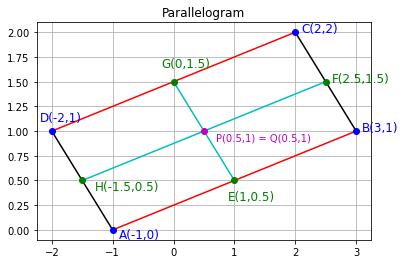
\includegraphics[width=\columnwidth]{parallelogram.png}
 \caption{The parallel lines are represented in red and black, and the initial vectors are represented in blue. The midpoints are represented in green, while the midpoints of $\vec{EG}$ and $\vec{FH}$ is shown in Magenta}
 \end{figure}
\end{document}
